\documentclass{article}


\def\Title{Software Design Document}
\def\Class{Software Engineering}
\def\Project{SE-Blackjack}
\def\Author{Sean Allred, Molly Domino, Joshua Kaminsky, Matthan Lee}
\def\SDPVersion{1.4}
\def\SRSVersion{1.3}
\def\TMVersion{1.2}
\def\SDDVersion{1.6}
\def\STPVersion{0.0}
\def\GUIVersion{0.0}
\def\CodeVersion{0.0}
\def\Version{\SDDVersion}
\title{\Title}
\author{\Author}
\date{\today}


\usepackage{graphicx}
\usepackage{verbatim}
\usepackage[margin=1in]{geometry}
\usepackage{fancyhdr}
\pagestyle{fancy}
%\lhead{\Title}
\rhead{\Project\\\Title\\Version \Version}









%For sorting
\usepackage{datatool}
\newcommand{\sortitem}[2]{%
  \DTLnewrow{list}%
  \DTLnewdbentry{list}{label}{#1}%
  \DTLnewdbentry{list}{description}{#2}%
}

\newenvironment{sortedlist}%
{%
  \DTLifdbexists{list}{\DTLcleardb{list}}{\DTLnewdb{list}}%
}%
{%
  \DTLsort{label}{list}%
  \begin{description}%
    \DTLforeach*{list}{\theLabel=label,\theDesc=description}{%
      \item [\theLabel] \theDesc
    }%
  \end{description}%
}

\newcommand{\setupintro}{
\renewcommand{\thepage}{}
\maketitle
\begin{center}
\large Version \Version \normalsize
\end{center}
\newpage
\setcounter{page}{1}
\renewcommand{\thepage}{\roman{page}}
\tableofcontents 
\newpage
\setcounter{page}{1}
\renewcommand{\thepage}{\arabic{page}}
}



%Specific for the SRS:
\setcounter{tocdepth}{3}
\setcounter{secnumdepth}{5}
\begin{document}
\setupintro



\section{Version History}
\begin{tabular}{|l|l|p{3.25in}|l|}
\hline
Date & Version & Description & Author \\\hline
Oct 1, 2012 & 1.0 & Initial construction of spreadsheet & Sean, Molly, and Mat\\\hline
Oct 1, 2012 & 1.1 &Construction and importation of flowcharts.& Mat \\\hline
Oct 2, 2012 & 1.2 &Construction and importation of data flow diagrams and dictionary entries.& Mat \\\hline
Oct 3, 2012 & 1.3 &Importation of pesudocode modules.& Mat \\\hline
Oct 3, 2012 & 1.4 &General maintenance of document and typesetting.& Josh and Mat \\\hline
Oct 31, 2012 & 1.5 & Diagrams updated.& Molly \\\hline
Oct 31, 2012 & 1.6 & Acronyms section added.  Section 3.3 changed to refer to section 3.1 as per customer instructions.& Josh\\\hline
\end{tabular}

\section{Introduction}

\subsection{Purpose}
The Software Design Document serves as a complete model of the Software.  It includes separated models for the designs of data, architectures, interfaces, and procedures.  This document will be shown to the customer in order to convey the concepts of the design before the software is released.  It also serves as a reference to the “``big picture'' design model for developers during the construction phase.

Data Design models describe the data involved in the software and give graphical representations of the data flow during program use.  These models are informed based on the particular nature of the data involved.  By modeling the flow of information, we can more clearly understand where information for a particular source comes from, and how the software interacts with it.  Also, it allows us to examine exactly what data the program inputs and outputs.

Architecture Design models provide a high-abstraction model of the software as a whole describe the flow of information through the software.  By focusing on the structural components of the software, we can follow input from interfaces as it filters through the software.  

Interface Design models describe the way the different modules of the software interact, as well as the way that external actors interact with the software.  Interface design will allow for smooth transmission of data when the time comes.  Additionally, if changes are made to the way interfaces function, then these models and architecture models will allow us to follow that change through our program.

The Procedural Design models describe structured programming concepts using graphical, tabular, and textual notations, which enable the designer to represent procedural detail that facilitates translation to code. This blueprint for implementation forms the basis for all subsequent software engineering work.  Furthermore, these models will allow for the programs functional flow to translate more directly into procedural coding steps.

\subsection{Scope}
This document codifies and outlines the project's data structures and represents their interactions with flow diagrams and high-level architectural representations.  It presents the program infrastructure that will be supporting these data elements and the interfaces that will allow them to be accessed and edited.  This document makes no attempt to outline specific segments of fully-constructed code or to model user test cases.  Additionally, this document does not include Data Flow Diagrams beyond level 1.

\subsection{Definitions, Acronyms, and Abbreviations}\label{Terms}

\subsubsection{Acronyms}
\begin{sortedlist}
\sortitem{GUI}{ Graphical User Interface}
%\sortitem{SME}{ Subject Matter Expert}
%\sortitem{FA}{ Functional Analyst}
%\sortitem{SA}{ Solutions Architect}
%\sortitem{DEV}{ Developer }
%\sortitem{QA}{ Quality Assurance }
\sortitem{SDP}{Software Development Plan}
\sortitem{SRS}{Software Requirements Specification}
\sortitem{TM}{Traceability Matrix}
\sortitem{SDD}{Software Design Document}
\sortitem{STP}{Software Test Procedure}
\end{sortedlist}

\subsubsection{Definitions}
\begin{sortedlist}
\sortitem{Player}{A person or AI participating in a game of blackjack}
\sortitem{User}{The human interfacing with the game}
\sortitem{Dealer}{The computer controlled player}
\sortitem{Test}{A formal practice of subjecting a piece of software to various conditions in order to ensure it functions.}
\sortitem{Hit}{A move in blackjack.  The person who makes the move is dealt a card from the deck}
\sortitem{Stand}{A move in blackjack.  This move signifies the end of the players turn.}
\sortitem{Blackjack}{The game of we are making our software to simulate.}
%\sortitem{Blackjack }{A hand in the game blackjack that consists of only an ace and a face card.  This hand is superior to all other non-blackjack hands.}
%\sortitem{Face Card}{Jack, Queen, or King}
\sortitem{Split}{A move in blackjack.  The user splits their hand into two separate hands, and makes a bet on the second hand equal to the initial bet.  The player then proceeds to play both hands separately.}
\sortitem{Subprogram}{A modular segment of code in the main program that performs a specific task.}
\sortitem{Gears}{A term for a subprogram dedicated entirely to computation.}
\sortitem{Main Program}{See section \ref{DataDefs}}
\sortitem{Main Program}{See section \ref{DataDefs}}
\sortitem{User Subprogram}{See section \ref{DataDefs}}
\sortitem{Computational Class}{See section \ref{DataDefs}}
\sortitem{Graphical User Interface}{See section \ref{DataDefs}}
%\sortitem{Coding}{The process of writing code.}
\end{sortedlist}

\subsubsection{Abbreviations}
\begin{sortedlist}
\sortitem{Sept}{September}
\sortitem{Oct}{October}
\sortitem{Dec}{December}
\end{sortedlist}


\subsection{References}

\begin{itemize}
\item SDP version \SDPVersion
\item SRS version \SRSVersion
\item TM version \TMVersion
\item STP version \STPVersion
\item GUI version \GUIVersion
\item Code version \CodeVersion
\item Glossary - see section \ref {Terms}
\item Other - Thank you to GitHub.com for allowing our team to collaborate online.  
\end{itemize}

\subsection{System Overview}
We are going to create a fully functional GUI based 1-player blackjack game.

\section{Data Design}

\subsection{Internal Data Structures}\label{DataDefs}
List/describe significant internal program data structures used to support the operation of the software.
\begin{itemize}
\item Card Handling 
\begin{itemize}
\item Deck $\rightarrow$ an ArrayList of paired enumerations called cards.  
\item Card $\rightarrow$ A paired enumeration of Suite/ Rank.  Hearts/Ace
\item Hand $\rightarrow$  when cards are dealt, they are added to a smaller arraylist called Hand.  This will also contain card enumerations.  
\begin{itemize}
\item There will need to be two data structures involving Hand.  One for the dealer and one for the player 
\end{itemize}
\item Discard$\rightarrow$an Arraylist containing all cards that have been used in play in an iteration.  When the Deck runs out, cards are removed from Discard and reshuffled to create a new Deck.  
\end{itemize}
\item Integer Balance $\rightarrow$holds the amount of money the user has at any time.
\item Integer Bet $\rightarrow$holds the amount of money the user places as a bet.
\item String Username $\rightarrow$holds the name the player inputs when the game begins
\item Statistics 
\begin{itemize}
\item Highest value won $\rightarrow$an integer value that saves the highest value bet won by the user.  Is initialized to 0.  
\item Highest value lost $\rightarrow$an integer value that saves the highest value bet lost by the user.  Is initialized to 0.
\item Wins/Losses $\rightarrow$Integer values that increment as a result of a hand of blackjack.  Wins increments by
\end{itemize}
\item GUI Data Structures
\begin{itemize}
\item Card Picture Library $\rightarrow$a static array containing references to images for each card.  
\item Card Back $\rightarrow$the reference to an image that will appear as the non-valued side to each card
\end{itemize}
\end{itemize}
\subsection{Data Flow Diagrams}

\subsubsection{Level 0}
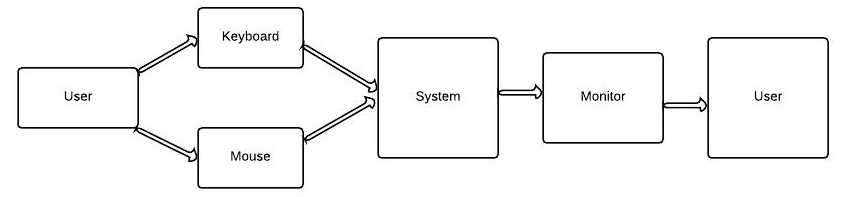
\includegraphics[width=\textwidth]{Level0Diagram}

\subsubsection{Level 1}
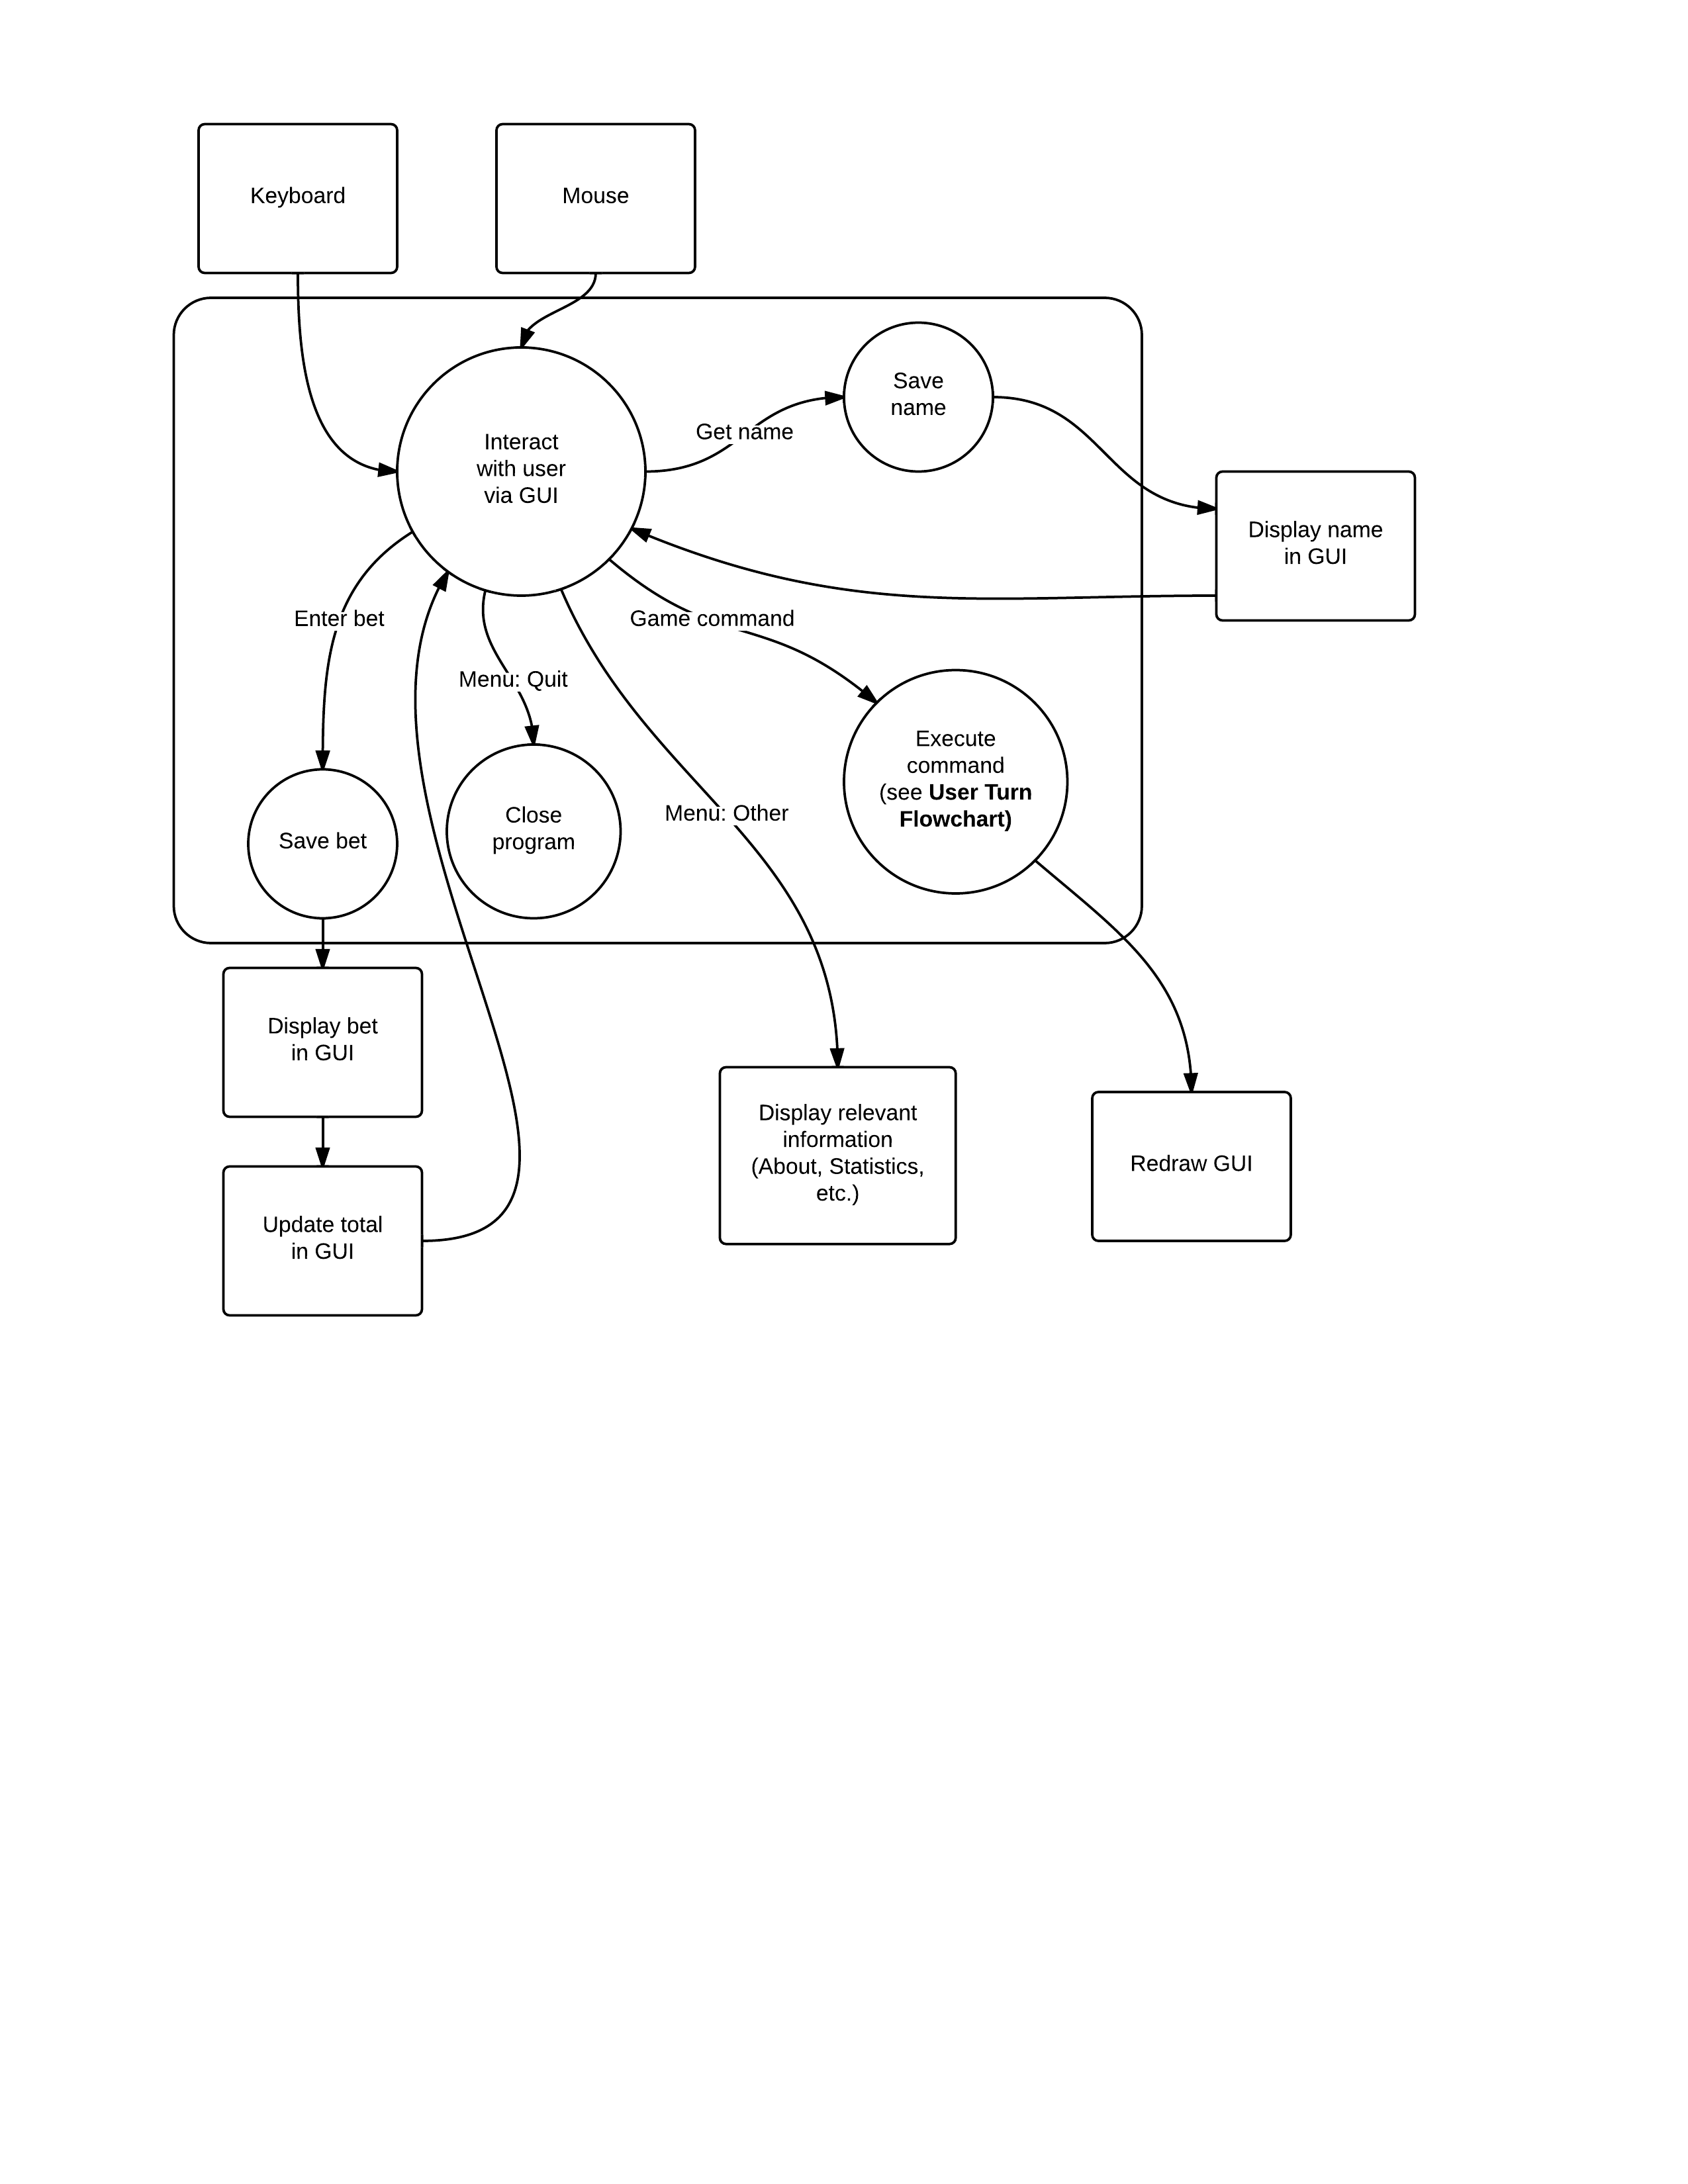
\includegraphics[width=\textwidth]{Level1DFD}


\subsection{Data Dictionary}

The information in this section has been covered in section \ref{DataDefs}.

\subsection{External System Interfaces}
\begin{itemize}
\item User passes arguments to Driver class via keyboard.
\item User passes mouse events to GUI via mouse.
\end{itemize}

 
\subsection{User Interfaces}

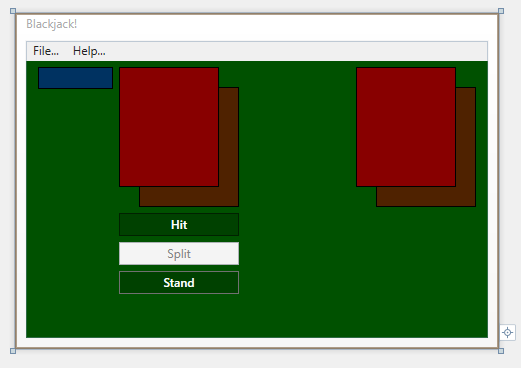
\includegraphics[width=\textwidth]{interface}

 

\section{Procedural Design}



\subsection{Blackjack Opening Flowchart}
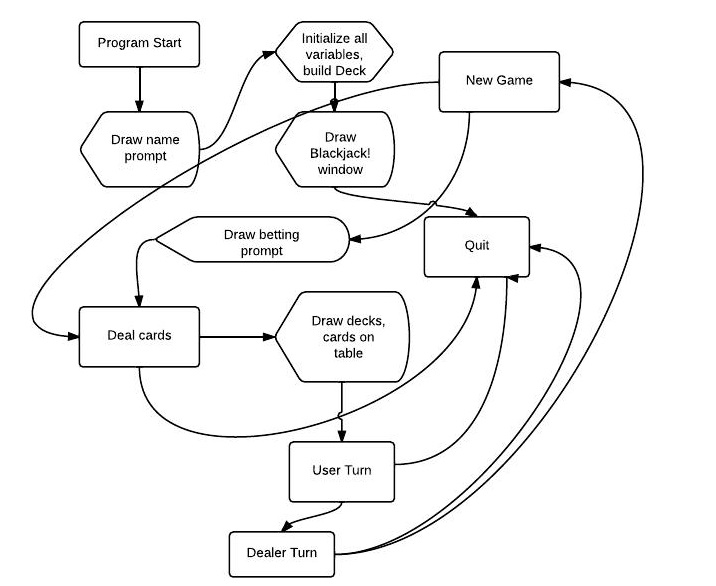
\includegraphics[width=\textwidth]{BlackjackOpeningFlowchart}

\subsection{User Turn Flowchart}
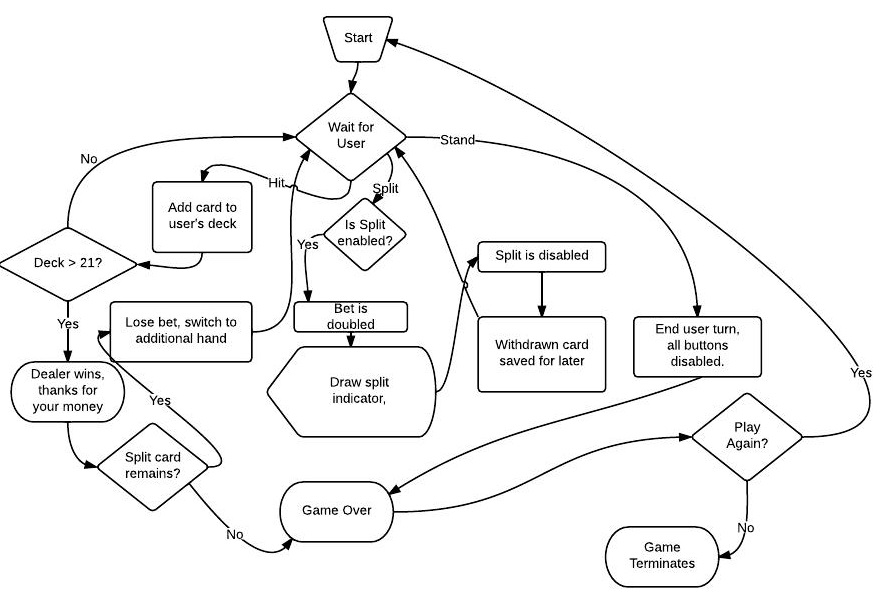
\includegraphics[width=\textwidth]{UserTurnFlowchart}


\begin{comment}
\subsection{Main Program startup pseudocode:}

•String name;
•GUI namePopup (JFrame input-listener, perhaps);
•double bank = 500.00;
•double bet = 0.00;
•int wins = 0;
•int losses = 0;
•Here we need to instantiate the entire ArrayList() of Card objects,
each with a unique face image.
•ArrayList<Cards>() hand = new ArrayList<>();
•ArrayList<Images>() images = new ArrayList<>();
images.add(new Image(“/resources/TwoOfHearts.png”);
images.add(new Image(“/resources/TwoOfClubs.png”);
images.add(new Image(“/resources/TwoOfDiamonds.png”);
images.add(new Image(“/resources/TwoOfSpades.png”);
…
images.add(new Image(“/resources/AceOfSpades.png”);
do (52) {
    i = 0;
    hand.add(new Card(images.get(i)));
    i++;
    }
/*
 * This psuedocode would create a 52-card ArrayList of Card objects, each with a uniquedoc
 * image associated with them.  I know there are more steps, like assigning them names
 * to allow comparison, et cetera, but this is just for starters.
*/

Graphical User Interface startup pseudocode:
•GUI blackjack (master Frame = new Frame(title = “Blackjack”);
•GUI fileMenu (new ComboBox(“New Game”, “Restart”, “Statistics”, “Exit”));
(drop-down File menu)
•GUI helpMenu (new ComboBox(“About”)); (drop-down Help menu)
•Label bettingBox (new Label = bet.toString());
•Label player (new Label = “PLAYER”)
•Label dealer (new Label = “DEALER”)
•Label userFunds (new Label = “Funds: ”+bank + “.”)
•Image dealerStack(new Image (“/resources/cardStack.png”)
•Button hit = new Button(enabled = false)
•Button split = new Button(enabled = false)
•Button stand = new Button(enabled = false)
•Tabletop userCards = new Tabletop();
•Tabletop dealerCards = new Tabletop();

Computational Class startup pseudocode:
•ArrayList<Card> userHand = new ArrayList<>();

•hand.shuffle()
•Card card = hand.get(random);
•userHand.add(card);
•userCards (that made-up Tabletop class) .play(card, faceup);
.play() should draw the card onscreen, face-up.

•card = hand.get(random);
•dealerHand.add(card);
•dealerCards.play(card, facedown);

•card = hand.get(random);
userHand.add(card);
userCards.play(card, faceup);

•card = hand.get(random);
•dealerHand.add(card);
dealerCards.play(card, facedown);
\end{comment}

\section{Miscellaneous}
The document contains no further items.

\end{document}